\scanpage{152}\mspage{7}%
A) The formalism of $Rf_!, f^!$ (combined with $Rf_*, Lf^{\alpha}$, $\overset{\mathbb{L}}{\otimes}$ and $\mathbb{R}\mathrm{Hom}$, ``the six operations'') implicitly carries within itself the definition of homology and the essential identity between homological and cohomological \unsure{functions}. \deleted{\unsure{E}} For the moment one has this formalism for quasi-coherent sheaves on schemes -- Hartshorne seminar -- for topological spaces and sheaves with arbitrary coefficients on them -- Verdier, Bourbaki talk -- and in the étale cohomology of schemes for ``discrete'' coefficients \inserted{(torsion or ``$l$-adic'')}
% Source guide below the parenthetic addition: long upper arm, short left descent beside premiers, and right upturn; no arrowhead. The separate lower crossed stem belongs to f in faisc.
\figure{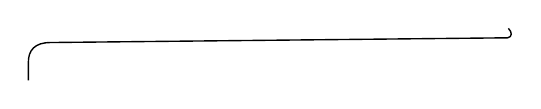
\begin{tikzpicture}[x=0.01cm,y=-0.01cm]
\draw[line width=0.5pt] (610,0) .. controls (615,5) and (615,11) .. (609,12)
 -- (28,18) .. controls (8,18) and (0,28) .. (0,43) -- (0,66);
\end{tikzpicture}}
\uline{prime \unsure{to the|to the} \deleted{\unsure{the|the}} residue characteristics} -- SGA 5 --
% The right guide lies above the added analytic case and descends from after SGA 5 into the space above the names. Its semicolon is reproduced inside the bend, not assigned an invented baseline order.
\figure{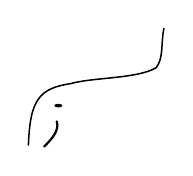
\begin{tikzpicture}[x=0.02cm,y=-0.02cm,line cap=round,line join=round]
\draw[line width=0.55pt] (89,2) .. controls (87,11) and (89,21) .. (84,27) .. controls (72,34) and (44,33) .. (30,37) .. controls (10,40) and (4,47) .. (3,76);
\fill (22,51) ellipse [x radius=2.6,y radius=1.15];
\draw[line width=0.8pt] (21,61) .. controls (23,67) and (17,73) .. (13,77);
\end{tikzpicture}}
\inserted{finally for coherent sheaves on analytic spaces -- Verdier-\unsure{Rüget|Ruget|Rüguet|Ruguet} --}
% The addition is slightly slanted in the source.
(The formalism remains to be developed in the crystalline context, and in characteristic $0$ in the context of stratified modules \inserted{with singularities}
% Guide immediately below singularités, with an uncertain detached point to its left below early stratifiés. The g descender above is separate from the guide.
\figure{\begin{tikzpicture}[x=0.01cm,y=-0.01cm]
\path[use as bounding box] (0,65) rectangle (577,136);
\node[inner sep=0pt] at (88,113) {\unsure{.}};
\draw[line width=0.5pt] (363,127) .. controls (353,96) and (359,79) .. (401,75)
 .. controls (423,71) and (437,72) .. (448,76)
 .. controls (491,94) and (544,98) .. (567,94);
\end{tikzpicture}}
in the manner of Deligne, with possibly -- over the field $\mathbb{C}$ -- Hodge structures into the bargain, finally in the context of motives; I am convinced that it is present
% The small doubtful point stands below the beginning of un, rather than after the word.
more or less everywhere else -- everywhere, \unsure{perhaps|perhaps}, where there is a formalism of a cohomological nature.) Working in étale cohomology on a \inserted{separated} scheme
% Guide immediately below séparé: curved left descent before de, rising arm, and small terminal hook at upper right.
\figure{\begin{tikzpicture}[x=0.02cm,y=-0.02cm,line cap=round,line join=round]
\draw[line width=0.55pt] (14,70) .. controls (3,55) and (3,40) .. (19,34) .. controls (40,25) and (82,19) .. (105,9) .. controls (114,5) and (110,0) .. (102,3);
\end{tikzpicture}}
of finite type over a field $k$, say,
% Detached point beneath the initial portion of avec; intent uncertain.
with a ring of \unsure{coefficients|coefficients} $\Lambda$ of \unsure{torsion} \unsure{prime} to \unsure{the} \unsure{characteristic}
% The last baseline is cut by the lower edge; no final punctuation is recoverable.
% archive sheet number: 152
